\externaldocument[-f]{c2_foundations}
\chapter{Experimental Setup}

This chapter presents the methodology used in this thesis. First, it is explained how different frameworks introduced in \autoref{chap:2} are put into use. Then, the algorithms used in data generation and inference is given in detail. The results from these experiments are presented in the succeeding chapter.

\section{The Model}
\begin{wrapfigure}{r}{3cm}
	\begin{center}
		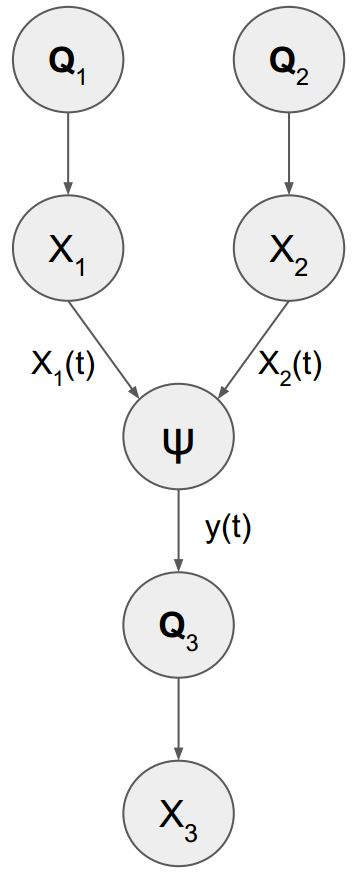
\includegraphics[width=2.5cm]{figures/h_model}
		\caption{Hierarchical model.}
	\end{center}
	\label{fig:h_model}
\end{wrapfigure} 
A detailed graphical model explored in this thesis is given in the \autoref{fig:h_model}. This model presents an intersection of continuous-time Bayesian network and partially observable Markov decision process frameworks. 
\begin{itemize}
	\item The transition models of the nodes $ X_1, X_2$ and $ X_3 $, and the dependencies between them are modelled as CTBN.
	\item The interaction of agent node $ X_3 $ and its environment is modelled as POMDP.
\end{itemize}

\subsection{CTBN Model}

The transition models of the nodes and the dependencies between them are modelled as continuous-time Bayesian network (CTBN), denoted by \textbf{X}. The network \textbf{X} represents a stohastic process over a structured multivariate state space $ \rchi = [\rchi_1, \rchi_2, \rchi_3] $. 

The parent nodes $X_{1}$ and $ X_{2} $ emits their states as messages. The dynamics  of these nodes are modelled as independent homogeneous continuous-time Markov processes $X_{i}(t)$, with binary-valued states $ \rchi_{i} = \left\lbrace 0, 1 \right\rbrace  $ for $ i \in \left\lbrace 1,2 \right\rbrace $. These processes are defined by transition intensity matrices $ \textbf{Q}_{i} $, which are in the following forms and assumed to be gamma distributed with shape and rate parameters $ \boldsymbol{\alpha} = [\alpha_0, \alpha_1] $ and $ \boldsymbol{\beta} = [\beta_0, \beta_1] $, respectively.
\begin{align}
\textbf{Q}_i &= 
\begin{bmatrix}
-q^i_{0} & q^i_{0} \\
q^i_{1} &  -q^i_{1}
\end{bmatrix}
\label{eq:Q_parents}\\
\textbf{Q}_{i} &\sim Gam(\boldsymbol{\alpha}^i, \boldsymbol{\beta}^i)\ \ for\ i \in \left\lbrace 1,2\right\rbrace \nonumber
\end{align}
It should be noted that in \autoref{eq:Q_parents}, the suffixes are simplified using the fact that $ q_{i} = \sum_{i \neq j} q_{i,j}$.

The agent  $ X_{3} $ is modelled as inhomogenouos continuous-time Markov process with binary states $ \rchi_{3} = \left\lbrace 0, 1 \right\rbrace  $ and set of actions $ a \in \left\lbrace a_0, a_1\right\rbrace  $, and set of transition intensity matrices which contains one matrix corresponding to each action, $ \textbf{\textit{Q}}_{3} = \left\lbrace \textbf{Q}_{a_{0}}, \textbf{Q}_{a_{1}} \right\rbrace $.
%\begin{equation}
%\textbf{Q}_{a_k} \sim Gam(\alpha_{a_k}, \beta_{a_k})
%\end{equation}

The dependencies are represented by set of parents for each node $ \textbf{U}_{X_{n}} = Par(X_n) $ and for the model shown in \autoref{fig:h_model} can be written as follows:
\begin{align*}
\textbf{U}_{X_{1}}, \textbf{U}_{X_{2}} & = \emptyset \\
\textbf{U}_{X_{3}} & = \left\lbrace X_1, X_2 \right\rbrace 
\end{align*}

\subsection{POMDP Model}
In a conventional POMDP scenario, there are two problem to be addressed, one is belief state update and the other is policy optimization. As mentioned in \autoref{sec:belief_POMDP}, in the problem at hand, the policy of agent $ X_3 $ is assumed to be optimal and given. Thus, the POMDP model of the agent only consists of belief state update. A detailed view of the agents interaction from POMDP framework perspective is given in the \autoref{fig:POMDP_pers}. \\
\textbf{SHOULD I ADD 'inspired by ...' WITH CITATION TO POMDP PAPER?}\\
\begin{figure}[htb]
	\begin{center}
		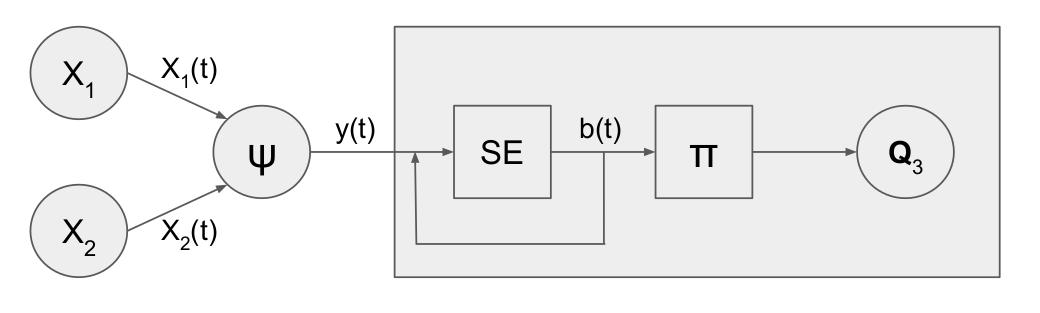
\includegraphics[width=.75\textwidth]{figures/POMDP_pers}
		\caption{Closer look to agent-environment interaction from the perspective of POMDP framework.}
		\label{fig:POMDP_pers}
	\end{center}
\end{figure}\\
The agent node $ X_3 $ does not have a direct access to the messages, but observes a translation of them. The observation model is defined as the likelihood of a translation given the parent messages.
\begin{equation}
\psi \coloneqq \operatorname{Pr}(y(t) \mid X_{1}(t), X_{2}(t))
\end{equation}
The state estimator (labelled as SE in \autoref{fig:POMDP_pers}) forms a belief over the parent states, $  b(x_{1}, x_{2}; t) $. 
\begin{equation}
b(x_{1}, x_{2}; t) = \operatorname{Pr}( X_{1}(t) = x_{1},  X_{2}(t) = x_{2}\mid y_{1}, ..., y_{t})
\end{equation}
Given the optimal policy, $ \pi(b(t)) $, the agent takes an action based on the belief state. In the setting described above, taking an action means to change its internal dynamics to the transition intensity matrix corresponding to that action.
\begin{align}
a(t) &= \pi(b(t))\\
\textbf{Q}_3(t) & = \textbf{\textit{Q}}_3[a(t)]
\end{align}
\textbf{WORK ON THESE NOTATIONS}\\

\subsubsection{POMDP Model with Exact Belief State Update}
Given the transition intensity matrices of parent nodes, $ \textbf{Q}_1 $ and $ \textbf{Q}_2 $, the belief state update poses a filtering problem for CTMPs (\autoref{sec:filtering_CTMC}). 

Consider a subsystem of CTBN model, consisting of only the parent nodes, $ X_1 $ and $ X_2 $. These two processes can be represented as one single \textit{joint} process, P, with joint state space $ \textit{P} = \left\lbrace (x_1, x_2)\right\rbrace  = \left\lbrace (0,0), (0,1), (1,0), (1,1)\right\rbrace  $. The transition intensity matrix of the new joint system, $ \textbf{Q}_P $ is obtained by amalgamation operation between $ \textbf{Q}_{1} $ and  $ \textbf{Q}_{2} $ \cite{Nodelman1995}.
%TODO x_1 and x_2 notation is not mentioned before, clarify!
\begin{equation}
\textbf{Q}_P = \textbf{Q}_{1} * \textbf{Q}_{2}
\end{equation}
\textbf{AMALGAMATION EXPLANATION AT APPENDIX?}\\
Consider discrete-time observations, denoted by $ y_{1}=y(t_{1}), ..., y_{N}=y(t_{N}) $. Following \autoref{eq:b_cont} and \autoref{eq:b_jump}, the belief state update is evaluated as
%TODO give initial condition
\begin{equation}
b(t) = b(0) \exp(t\textbf{Q}_P)
\end{equation}
with reset condition at discrete times of observation $ y_{t} $ 
\begin{align}
b(x_{i}; t_{N}) &= Z_{N}^{-1}\ {\operatorname{Pr}(y_{N} \mid X(t_{N})=x_{i})}\ {b(x_{i}; t_{N}^{-})} \\ & = Z_{N}^{-1}\ \psi \ {b(x_{i}; t_{N}^{-})}
\end{align}
where $ Z_{N} = \sum_{x_{i}\in \rchi} \operatorname{Pr}(y_{N} \mid X(t_{N})=x_{i})\ b(x_{i}; t_{N}^{-}) $ is the normalization factor.

\subsubsection{POMDP Model with Belief State Update Using Particle Filter}

\scalebox{1}{\begin{algorithm}[H]
		\KwIn{Measurement data $ y_{k} $ at time $ t_{k} $, set of particles $\textbf{p}^{k-1} $, estimated $ \hat{Q} $}
		\KwResult{New set of particles $ \textbf{p}^{k} $, representing $ b(t_{k}) $}
		\vspace{+4pt}
		\begin{algorithmic}[1]
			\FOR{$p_{m} \in \textbf{p}^{k-1}$}
			\STATE {$p_{m} = \left\lbrace x_{m}, \hat{Q}\right\rbrace \leftarrow Propagate\ particle\ through\ marginal\ process\ model\ from\ t_{k-1}\ to\ t_{k}$ }
			\STATE{$w_{m} \leftarrow p(y_{k} \mid X(t_{k})=x_{m}) $} 
			\tcp*[h] {observation likelihood}
			\STATE {$\hat{Q} \leftarrow sufficient\ statistics\ added\ from\  p_{m}[t_{k-1}, t_{k}]$}
			\ENDFOR
			\STATE{$ w_{m} \leftarrow \frac{w_{m}}{\sum_{m} w_{m}}$} \tcp*[h]{normalize weights}
			\FOR{$ p_{m} \in \textbf{p}_{k} $} 
			\STATE{$ p_{m} \leftarrow Sample\ from\ p_{k}\ with\ probabilities\ w_{m}\ with\ replacement$}
			\ENDFOR
		\end{algorithmic}
		\caption{Marginal particle filter}
\end{algorithm}}
\subsubsection{Optimal Policy}

The optimal policy is defined as a polynomial function of belief state.
\begin{align}
\pi(b(t)) = \textbf{w}\ b(t)^T
\end{align}
where \textbf{w} is a row vector of weights.\\
\textbf{INCONSISTENT WITH NOTATION USED BEFORE}

\section{Data Generation}
\subsection{Sampling Trajectories}
\subsubsection{Gillespie Algorithm}
\subsubsection{Thinning Algorithm}
\section{Inference of Observation Model}
Our dataset contains a number of trajectories from all the nodes involved in the communication. $ \textbf{D} = \left\lbrace D_{1},..., D_{N}\right\rbrace $. Every trajectory comprises of state transitions in time interval $  [0, T] $, and the times of these transitions.


\section{Parameters}

\paragraph{Marginalized Likelihood Function} 
Let $ X $ be a homogenous CTMP. For convenience, it is assumed to be binary-valued, $ \rchi = \left\lbrace x_{0}, x_{1} \right\rbrace $. The transition intensity matrix can be written in the following form:
\begin{equation}
\textbf{Q} = 
\begin{bmatrix}
-q_{0} & q_{0} \\
q_{1} & -q_{1}
\end{bmatrix}
\end{equation}
where the transition intensities $ q_{0} $ and $ q_{1} $ are gamma-distributed with parameters $ \alpha_{0}$, $ \beta_{0} $ and $ \alpha_{1} $, $ \beta_{1} $, respectively. The marginal likelihood of a sample trajectory $ X^{[0,T]} $ can be written as follows:
\begin{align}
P(X^{[0, T]}) & = \int  P(X^{[0, T]}\mid Q)P(Q) dQ \nonumber\\ & = \int_{0}^{\infty} \left( \prod_{x} \exp(-q_{x}T_{x}) \prod_{x'} q_{xx'}^{M[x, x']}\right) \frac{\beta_{xx'}^{\alpha_{xx'}}{q_{xx'}^{\alpha_{xx'}-1}}\exp(-\beta_{xx'}q_{xx'})}{\Gamma(\alpha_{xx'})} \ dq_{xx'} \nonumber\\ & = \prod_{i\in{0,1}}\int_{0}^{\infty} q_{i}^{M[x_{i}]} \ \exp(-q_{i}T[x_{i}]) \  \frac{\beta_{i}^{\alpha_{i}} \ q_{i}^{\alpha_{i}-1}\ \exp(-\beta_{i}q_{i})}{\Gamma(\alpha_{i})} \ dq_{i} \nonumber\\ & = \prod_{i\in{0,1}} \frac{\beta_{i}^{\alpha_{i}}}{\Gamma(\alpha_{i})} \int_{0}^{\infty} q_{i}^{M[x_{i}] + \alpha_{i} -1} \ \exp(-q_{i}(T[x_{i}]+\beta_{i})) \ dq_{i} \\ & = \prod_{i\in{0,1}} \frac{\beta_{i}^{\alpha_{i}}}{\Gamma(\alpha_{i})} \left( -(T_{i}+\beta_{i})^{M[x_{i}] + \alpha_{i}}\ \Gamma(M[x_{i}] + \alpha_{i}, \ q_{i}(T[x_{i}]+\beta_{i})) \right) \Big|_0^\infty  \\ & = \prod_{i\in{0,1}} \frac{\beta_{i}^{\alpha_{i}}}{\Gamma(\alpha_{i})} \left( (T[x_{i}]+\beta_{i})^{M[x_{i}] + \alpha_{i}}\ \Gamma(M[x_{i}] + \alpha_{i}) \right)
\label{eq:Marg_traj}
\end{align}.
%
%where $ T[x_{i}] $, the amount of time spent in state $ [x_{i}] $, $ M[x_{i},x_{j}] $ the number of transitions from state $ x_{i} $ to $ x_{j} $ and  $ M[x_{i}] = \sum_{i\neq j}M[x_{i},x_{j}] $.\\

%From Eq.11, the integral is solved using computer algebra system WolframAlpha as follows:
%\begin{align}
%\int x^{a} \ \exp(-xb) \ dx = -b^{-a-1} \ \Gamma(a+1, \ bx) + C
%\label{eq:integral}
%\end{align}
%
%Plugging Eq.\ref{eq:Marg_traj} in Eq.\ref{eq:Marg_llh} for both $ X_{1} $ and $ X_{2} $:
%\begin{align}
%\begin{split}
%P(\textit{D} \mid \pi, \Phi ) = P(X_{3}^{[0, T]}\mid Q_{3}^{[0, T]}) \prod_{x_{1}\in{0,1}} \frac{\beta_{x_{1}}^{\alpha_{x_{1}}}}{\Gamma(\alpha_{x_{1}})} \ (T_{x_{1}}+\beta_{x_{1}})^{M_{x_{1}} + \alpha_{x_{1}}}\ \Gamma(M_{x_{1}} + \alpha_{x_{1}})  \\  \prod_{x_{2}\in{0,1}} \frac{\beta_{x_{2}}^{\alpha_{x_{2}}}}{\Gamma(\alpha_{x_{2}})} \ (T_{x_{2}}+\beta_{x_{2}})^{M_{x_{2}} + \alpha_{x_{2}}}\ \Gamma(M_{x_{2}} + \alpha_{x_{2}})
%\label{eq:Marg_llh_final}
%\end{split}
%\end{align}
